%\documentclass[first,firstsupp,handout,compress,notes,navigation]{ETHclass} 
%\documentclass[first,firstsupp,handout,notes]{ETHclass} 
\documentclass[first,firstsupp]{ETHclass} % handout
%\documentclass{ETHclass} 
%\documentclass[first,firstsupp,notes]{ETHclass} 
%\documentclass[first,firstsupp]{ETHclass}
% 
% Options for beamer:
%
% 9,10,11,12,13,14,17pt  Fontsizes
% 
% compress: navigation bar becomes smaller
% t       : place contents of frames on top (alternative: b,c)
% handout : handoutversion
% notes   : show notes
% notes=onlyslideswithnotes
%
%hyperref={bookmarksopen,bookmarksnumbered} : Needed for menues in
%                                             acrobat. Also need
%                                             pdftex as option or 
%                                             compile with
% pdflatex '\PassOptionsToPackage{pdftex,bookmarksopen,bookmarksnumbered}{hyperref} \input{file}'
% 
\usepackage{etex}
\usepackage{beamerseminar}
\usepackage{lmodern}
\usepackage{listings}
\usepackage{tikz}
\usepackage{verbatim}
\usepackage{wasysym}
\usepackage{bm}
\usetikzlibrary{arrows,shapes}

\tikzset{
    state/.style={
        rectangle,
        rounded corners,
        draw=black, very thick,
        minimum height=2em,
        inner sep=2pt,
        text centered,
    },
                                                                                     }


% \usepackage{amssymb}
% \usepackage{enumitem} % Strange
%\usepackage[accumulated]{beamerseminar}
                                % remove ``accumulated'' option
                                % for original behaviour
% \usepackage{beamerbasenotes}
% \usepackage{ragged2e} 
\usepackage{amsmath}
\usepackage{caption}
\usepackage{xcolor}
\usepackage{multicol}
\captionsetup[figure]{labelformat=empty}
\captionsetup[table]{labelformat=empty}

\newcommand{\R}{\mathbb{R}}
\newcommand{\E}{\mathbb{E}}
\newcommand{\ML}{\mathbb{L}}
\newcommand{\wv}{\bm{w}}
\newcommand{\xv}{\bm{x}}
\newcommand{\vv}{\bm{v}}
\newcommand{\Qv}{\bm{Q}}
\newcommand{\alphav}{\bm{\alpha}}
\newcommand{\deltav}{\bm{\delta}}
\newcommand{\chiv}{\bm{\chi}}
\DeclareMathOperator{\st}{\textrm{s.t.}}


%\setbeamertemplate{note page}[plain] 
%\setbeameroption{notes on second screen}
% 
% \usepackage[pdf]{pstricks}
% 
% %\setbeamertemplate{note page}[plain] 
% \setbeamertemplate{note page}{\ \\[.3cm]
% \textbf{\color{blue}Notes:}\\%[0.1cm]
% {\footnotesize %\tiny
% \insertnote}}
% %\setbeameroption{notes on second screen}
% 
% \usepackage{multimedia}
% 
\setbeamertemplate{navigation symbols}{} % suppresses all navigation symbols:
% \setbeamertemplate{navigation symbols}[horizontal] % Organizes the navigation symbols horizontally.
% \setbeamertemplate{navigation symbols}[vertical] % Organizes the navigation symbols vertically.
% \setbeamertemplate{navigation symbols}[only frame symbol] % Shows only the navigational symbol for navigating frames.
% 
\setparametertextfont{\scriptsize}
\setlabelfont{\scriptsize}
\setlength{\stockheight}{\paperheight}
% 
\title{Primal estimated sub-gradient solver for SVM}
\author{\small Lei Zhong}
\institute{\small Advanced Topics in Machine Learning}
\date{\tiny \textbf{Nov. 4, 2014}} 
% 
\let\Tiny=\tiny
\setbeamertemplate{itemize item}{\textbullet} 
\setbeamertemplate{itemize subitem}{$\rightarrow$} % \lozenge \heartsuit \diamondsuit \bigstar \clubsuit \spadesuit \square \Box \small $\bigstar$
\setbeamertemplate{sections/subsections in toc}[ball]
\setbeamertemplate{items}[ball]
%
\newcommand{\titleslide}{{%{{\usebackgroundtemplate{
\includegraphics[width=\paperwidth,height=\paperheight]{images/titleslide}}
\begin{frame}
 	% \frametitle{$ $} % 
 	\frametitle{Outline}
	\tableofcontents[currentsection, currentsubsection]
\end{frame}}}
%
\definecolor{dkgreen}{rgb}{0,0.6,0}
\definecolor{gray}{rgb}{0.5,0.5,0.5}
\definecolor{mauve}{rgb}{0.58,0,0.82}
%
\lstset{
	language=Java, %[Sharp]C, 				% c-sharp programming language
	numbers=left,					% where to put the line-numbers
	numberstyle=\tiny\color{gray},	% the style that is used for the line-numbers
	keywordstyle=\color{blue}\bfseries,	% keyword style
	keywordstyle=\color{blue},		% keyword style
	commentstyle=\color{dkgreen},	% comment style
	stringstyle=\color{mauve},		% string literal style
	stepnumber=1,					% the step between two line-numbers. If it's 1, each line 
									% will be numbered
	numbersep=5pt,					% how far the line-numbers are from the code
	tabsize=4,						% sets default tabsize to 2 spaces
	basicstyle=\small				% the size of the fonts that are used for the code	
}

\title{Primal estimated sub-gradient solver for SVM}

\begin{document}

\begin{comment}
unconstrained case is nice

iteration cost of SDCA, iteration cost d

SMO
\end{comment}

\begin{frame}
  	\maketitle
\end{frame}
%
\institute{\it \tiny{}}
\date{Nov. 4, 2014}
\author{\it Lei Zhong}
\title{\today \hspace{3.8cm} \arabic{page}}
%
\section{Introduction and Background}

\begin{frame}[fragile]
    \frametitle{Introduction}
     
    \begin{block}
    %\[
    %    {\bf w}^{(t)}=\Pi_K({\bf w}^{(t-1)}-\eta_t{\bf \chi_t})
    %\]
    \end{block}
    \begin{itemize}
        \item[(a)] $\Pi_K$ is the orthogonal projection on $K$
        \item[(b)] $\bf \chi_t$ is subgradient of $f$ at $\bf w}^{(t-1)}$
        \item[(c)] $\|\bf \chi_t\|^2 \le $
    \end{itemize}
\end{frame}

\subsection{Stable Matching}
\begin{frame}[fragile]
    \frametitle{Stable Matching}
    \begin{block}{Definition}
        \begin{itemize}
            \item Given two sets of {\color{blue} elements} with their set of {\color{blue} preferences}.
            \item A matching is a {\color{blue} mapping} from the elements of one set to the elements of the other set. 
            \item A matching is {\color{blue} stable} if there is no {\color{blue} blocking pair}.
        \end{itemize}
    \end{block}
\end{frame}

\tableofcontents

\section{Introduction}
\begin{frame}[fragile]
    \frametitle{Motivating example}
    \begin{figure}[htbp]
        \centering
        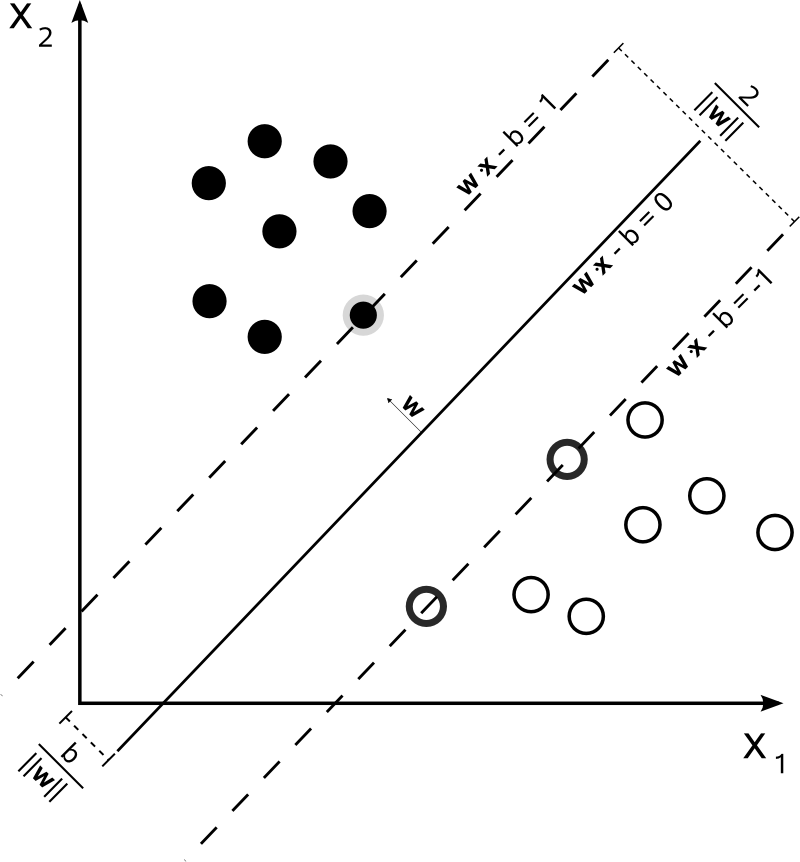
\includegraphics[height=0.8\textheight, width=0.7\textwidth]{images/svm_ex.png}
    \end{figure}
\end{frame}

\begin{frame}{Family Support Machine}
    \begin{figure}[htbp]
        \centering
        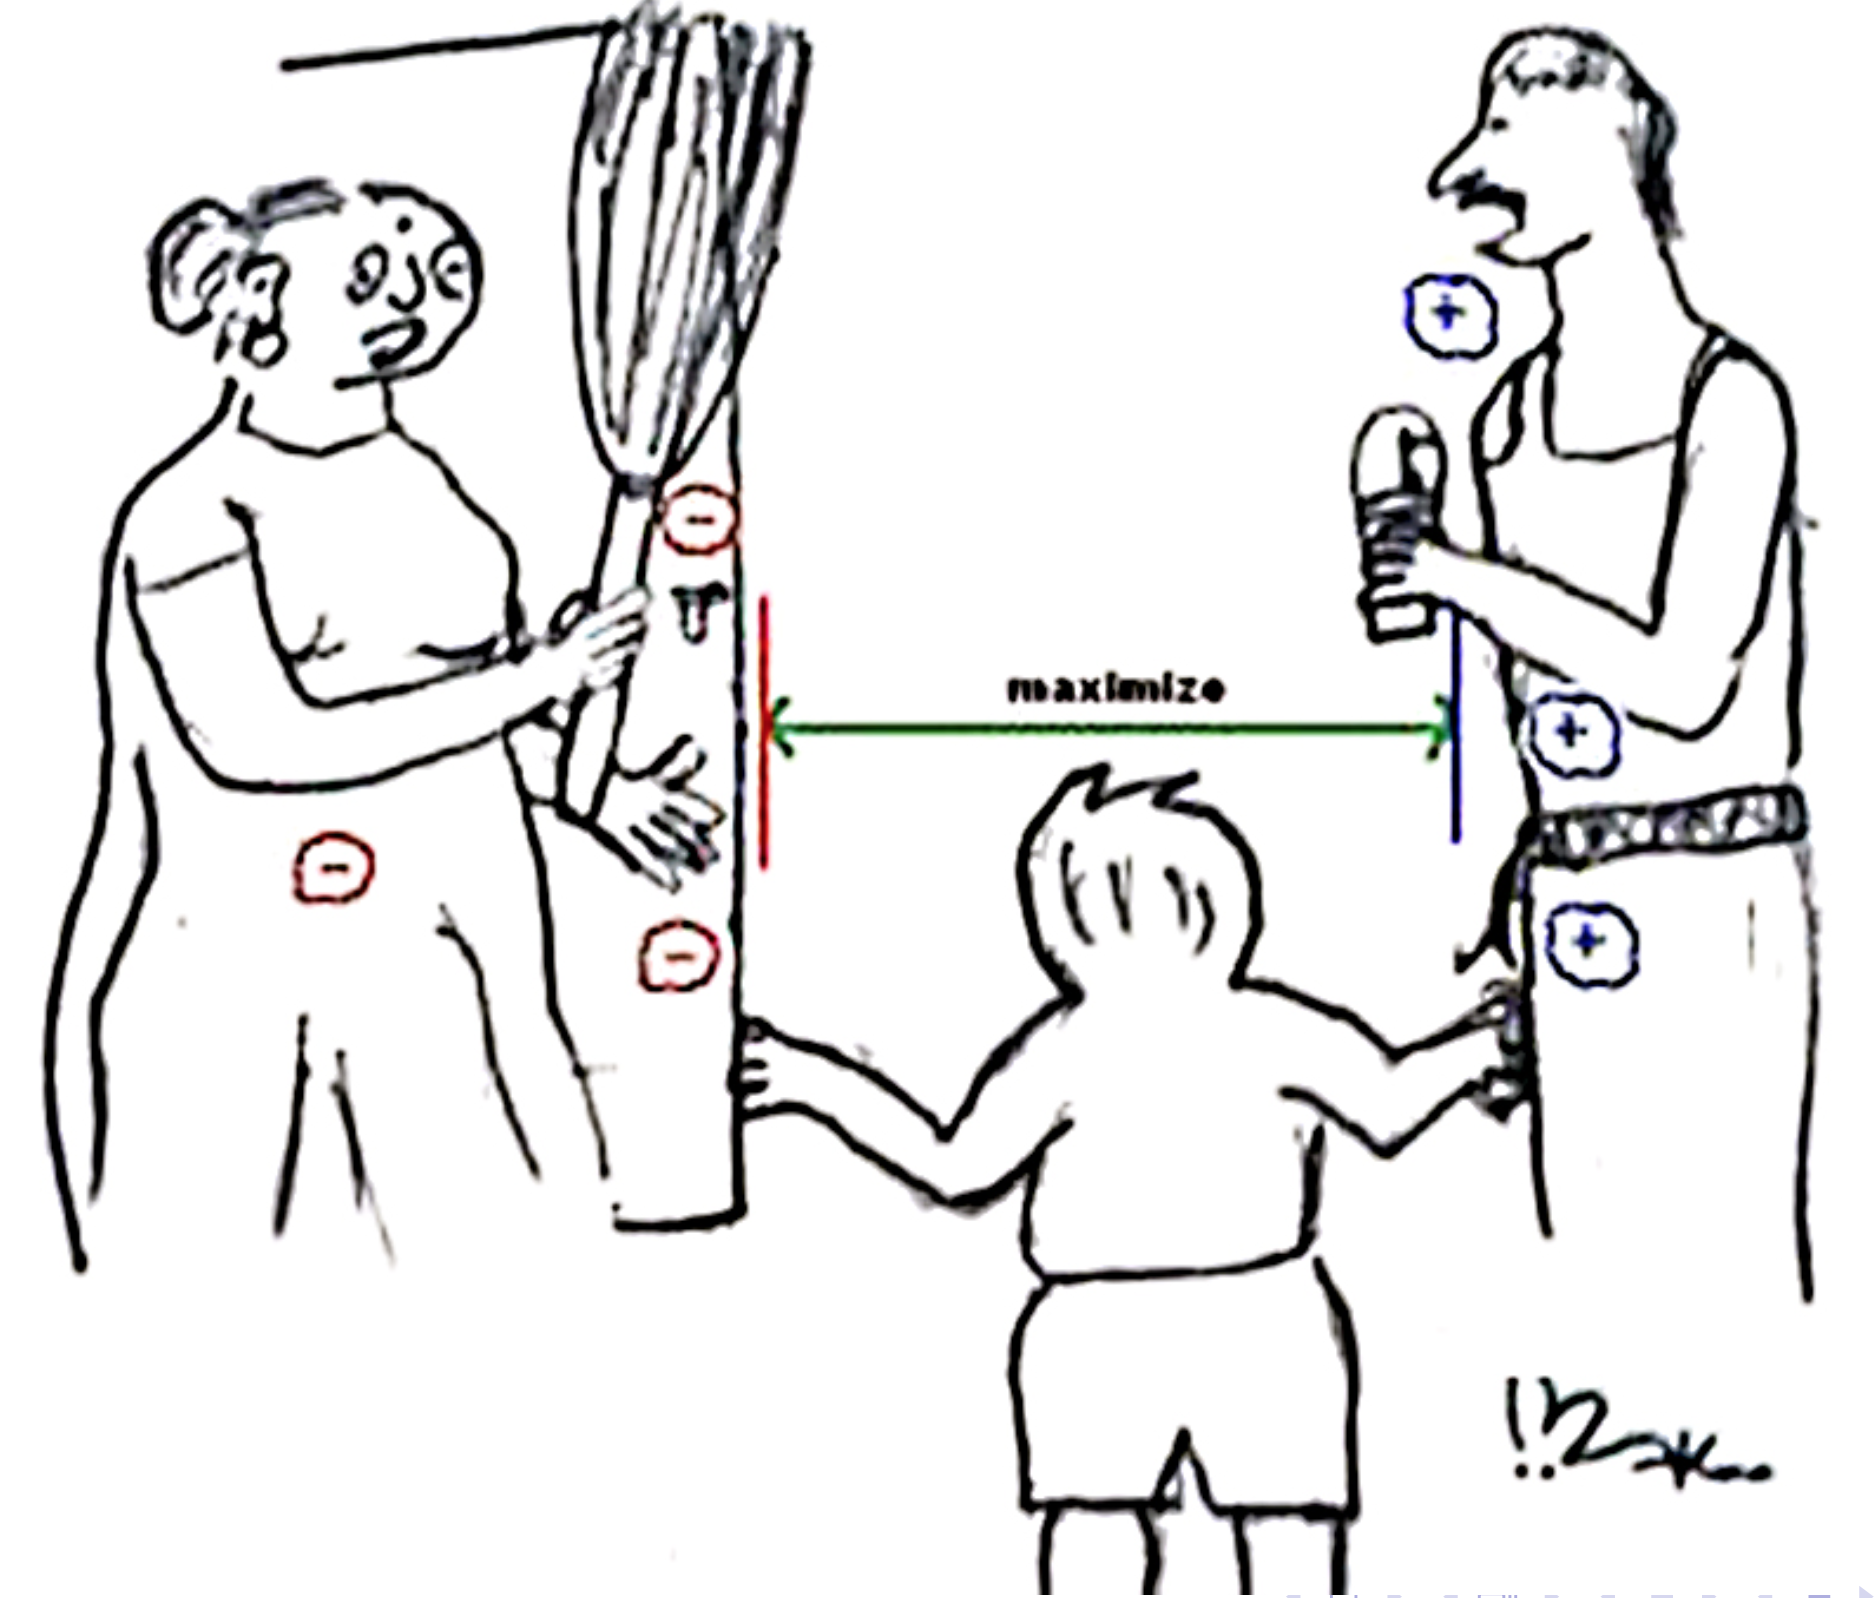
\includegraphics[height=0.6\textheight, width=0.7\textwidth]{images/family.png}
    \end{figure}
    From Peter Richt\'arik's slides
\end{frame}

\begin{frame}{Support Vector Machine: Primal Problem}
    Data: 
    \[
        \{(\xv_i,y_i)\in \R^d \times \{+1, -1\}: i\in S \overset{def}{=} \{1,2,\ldots,n\}\}
    \]
    \begin{itemize}
        \item[$\rhd$] Example: $\xv_1,\ldots,\xv_n$ (assumption: $\max_i\|\xv_i\|_2\le R$)
        \item[$\rhd$] Labels: $y_i \in\{+1,-1\}$
    \end{itemize}
    {\color{red} Optimization formulation of SVM:}
    \[
        \min_{\wv\in\R^d} \{ f(\wv):= \hat{L}_S(\wv)+\frac {\lambda} {2} \|\wv\|^2 \}
    \]
    where 
    \begin{itemize}
        \item[$\rhd$] $\hat{L}_A(\wv) \overset{def}{=} \frac{1}{|A|} \sum_{i\in A} L_i$ (average loss on examples in A)
    \end{itemize}
\end{frame}

\begin{frame}{Loss Function and Subgradient}
    \begin{block}{Definition}
        \begin{itemize}
            \item Loss: $L_i := \ell(\langle \xv_i, \wv \rangle, y_i)$

            \item Subgradient: $l'(\langle \xv_i, \wv \rangle, y_i)$ with $\|l'\| \le \mathbb{L}$
        \end{itemize}
    \end{block}
    Use the notation $z=\langle \wv, \xv_i\rangle$, sample loss functions:
    \begin{table}[h]
        \begin{tabular}{|l|l|}
            \hline
            Loss function & Subgradient  \\ \hline
            $l(z,y_i) = \max\{0,1-y_i z\}$ & $l' = \left\{
            \begin{matrix} -y_i x_i & \text{if } y_i z<1 \\ 
            0 & \text{otherwise}
            \end{matrix}
        \right\}$ \\ \hline
        $l(z,y_i) = \log(1+e^{-y_iz})$ & $l' = -\frac{y_i}{1+e^{y_i z}}\xv_i$\\ \hline
        $l(z,y_i) = \max\{0, | y_i - z| - \epsilon\}$ & $l'=\left\{ 
        \begin{matrix}
            \xv_i & \text{if } z-y_i > \epsilon \\
            -\xv_i & \text{if } y_i-z > \epsilon \\
            \bm{0} & \text{otherwise}
        \end{matrix}
        \right\}$ \\ \hline
        \end{tabular}
    \end{table}
\end{frame}


\section{Convergence analysis}
\subsection{Classical analysis}
\subsection{New analysis}
\subsection{}


\section{Experiments - outperforms state-of-the-art}
\begin{frame}{Experiments}
    \begin{itemize}
        \item 3 datasets (provided by Joachims) 
            \begin{itemize}
                \item Reuters CCAT (800K examples, 47k features)
                \item Covertype (581k examples, 54 features)
                \item Physics ArXiv (62k examples, 100k features)
            \end{itemize}
        \item 4 competing algorithms
            \begin{itemize}
                \item SVM-Perf (Joachims'06)
                \item SVM-light (Joachims)
                \item Norma (Kivinen, Smola, Williamson '02)
                \item Zhang'04 (stochastic gradient descent)
            \end{itemize}
    \end{itemize}
\end{frame}

\begin{frame}{Linear kernels}
\begin{table}[ht]
    \centering
    \begin{tabular}{l|l|l|l|l|l}
            \hline
            Dataset & Training & Testing & Features & Sparsity(\%) & $\lambda$ \\ \hline 
            astro-ph & 29,882 & 32,487 & 99,757 & 0.08 & $5\times 10^{-5}$ \\ 
            CCAT & 781,265 & 23,149 & 47,236 & 0.16 & $10^{-4}$ \\ 
            cov1 & 522,911 & 58,101 & 54 & 22.22 & $10^{-6}$ \\ \hline
        \end{tabular}
    \end{table}
\end{frame}

\begin{frame}{Linear kernels}
\begin{table}[ht]
    \centering
    \begin{tabular}{lllll}
            \hline
            Dataset & Pegasos & SDCA & SVM-Perf & LASVM \\ \hline 
            astro-ph & 0.04s(3.56\%) & 0.03s(3.49\%) & 0.1s(3.39\%) & 54s(3.65\%) \\ 
            CCAT & 0.16s(6.16\%) & 0.36s(6.57\%) & 3.6s(5.93\%) & $>$18000 s  \\ 
            cov1 & 0.32s(23.2\%) & 0.20s(22.9\%) & 4.2s(23.9\%) & 210s(23.8\%) \\ \hline
        \end{tabular}
    \end{table}
\end{frame}

\begin{frame}{Comparison of linear SVM optimizers}
    \begin{figure}[htbp]
        \centering
        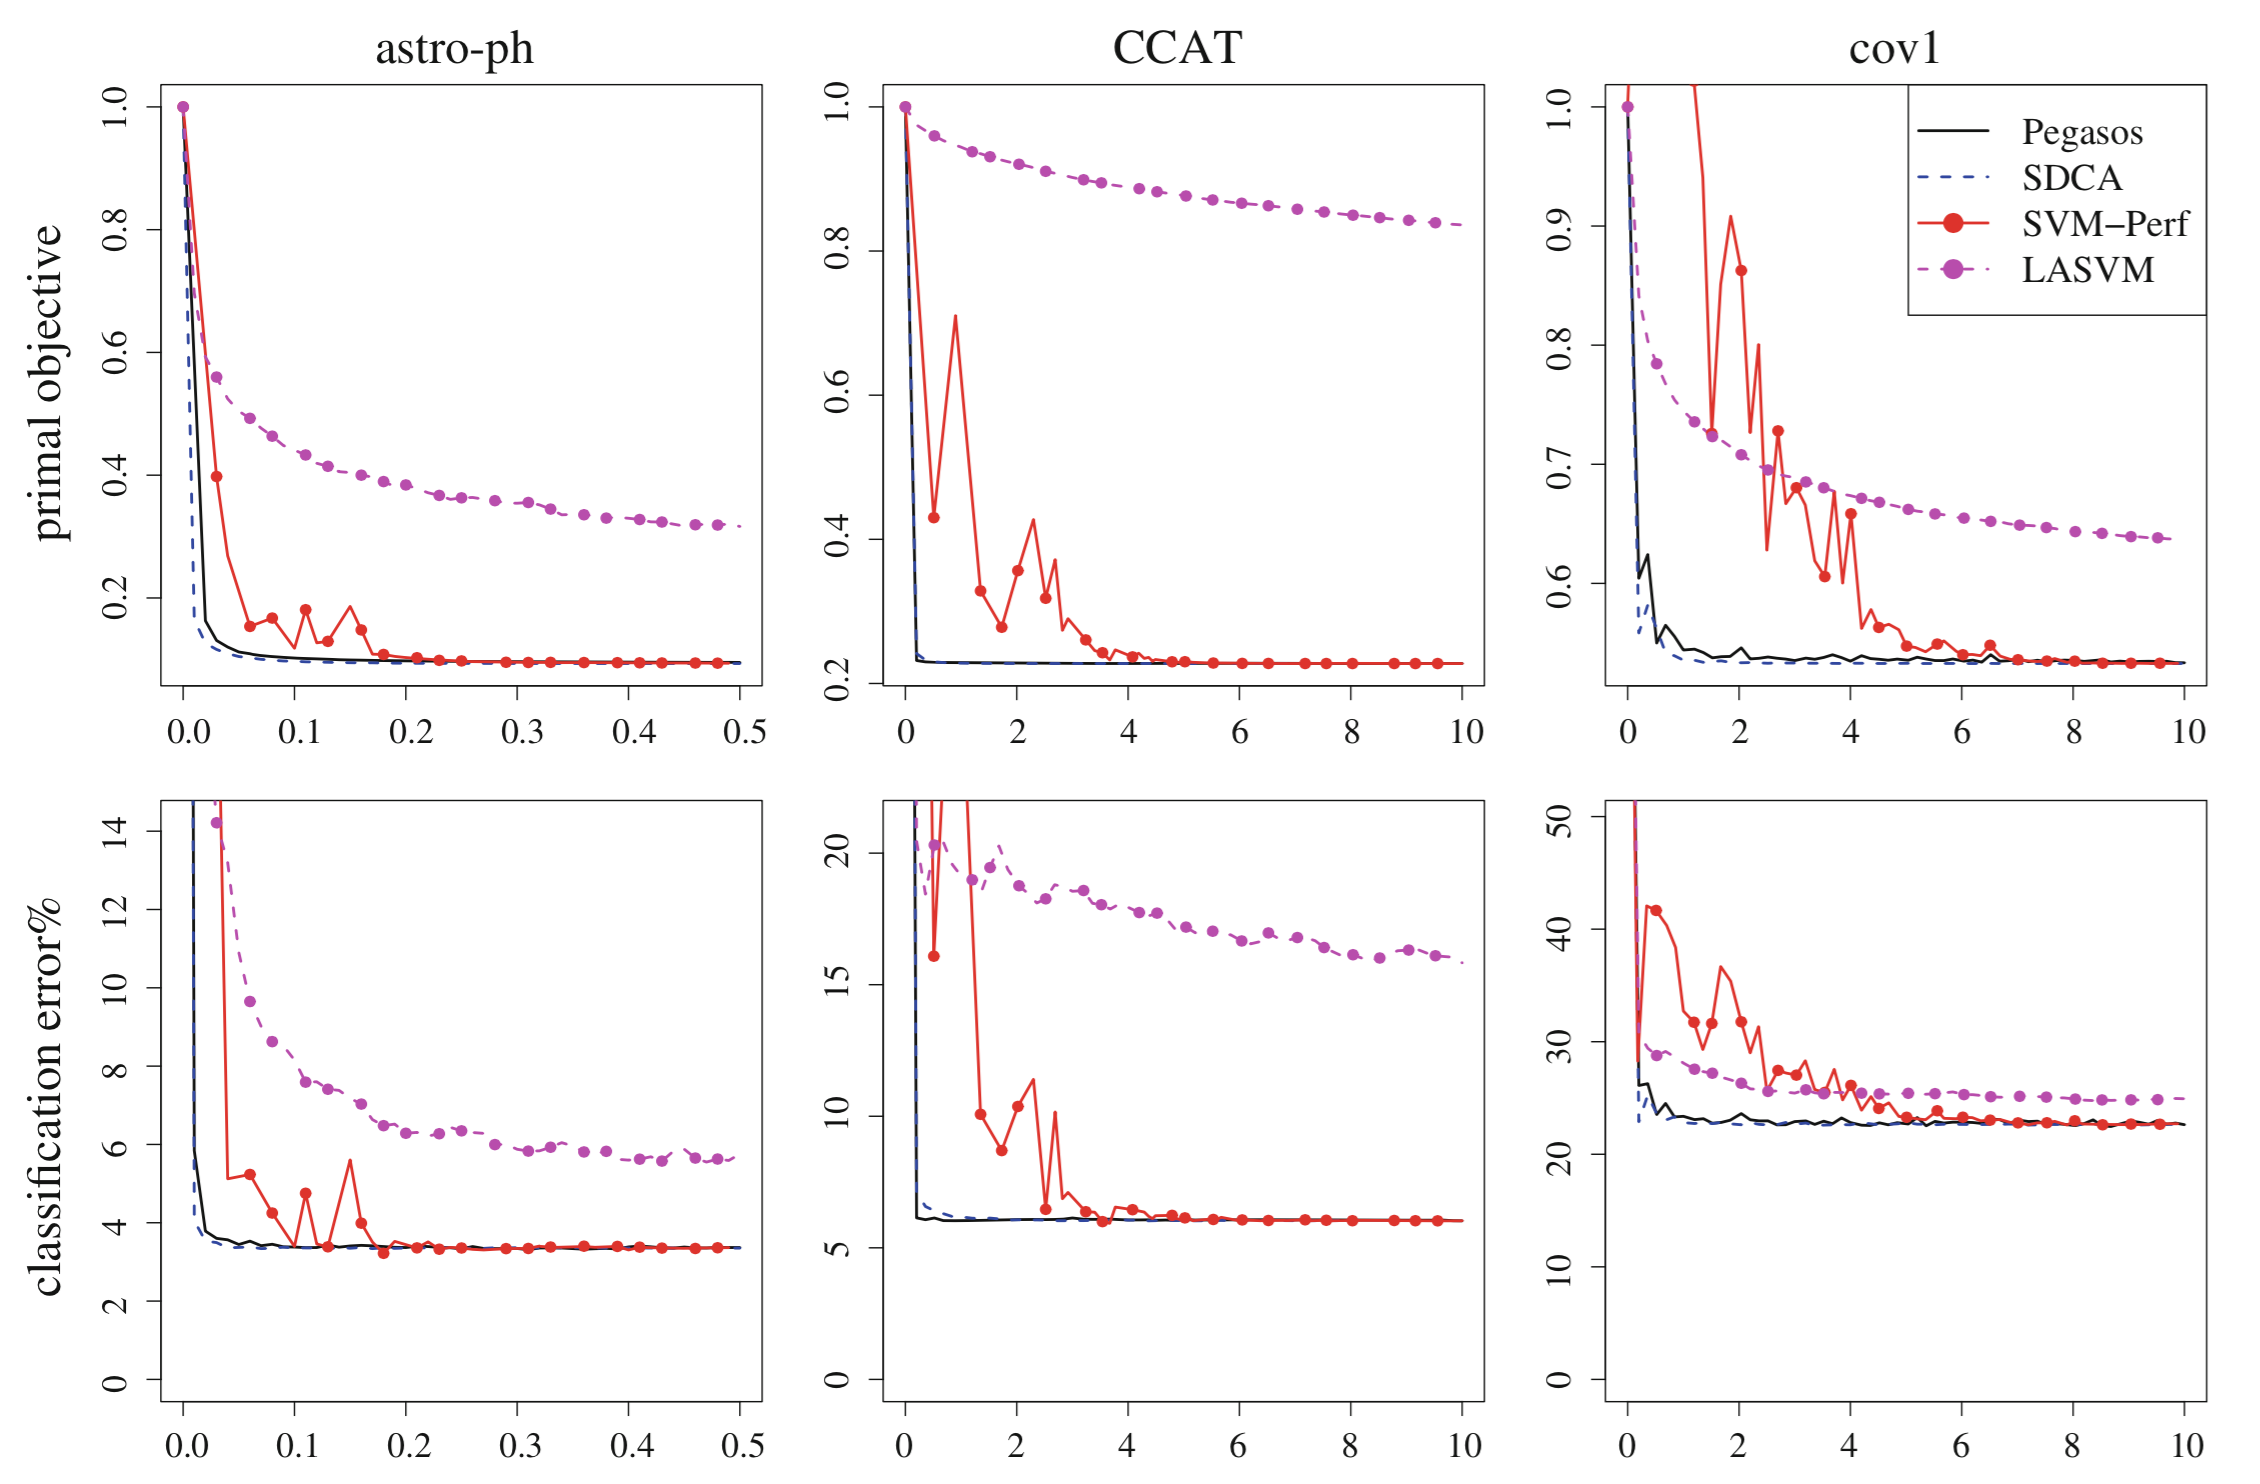
\includegraphics[height=0.7\textheight, width=\textwidth]{images/comp1.png}
    \end{figure}
\end{frame}

\begin{frame}{Effect of regularization parameter $\lambda$}
    \begin{figure}[htbp]
        \centering
        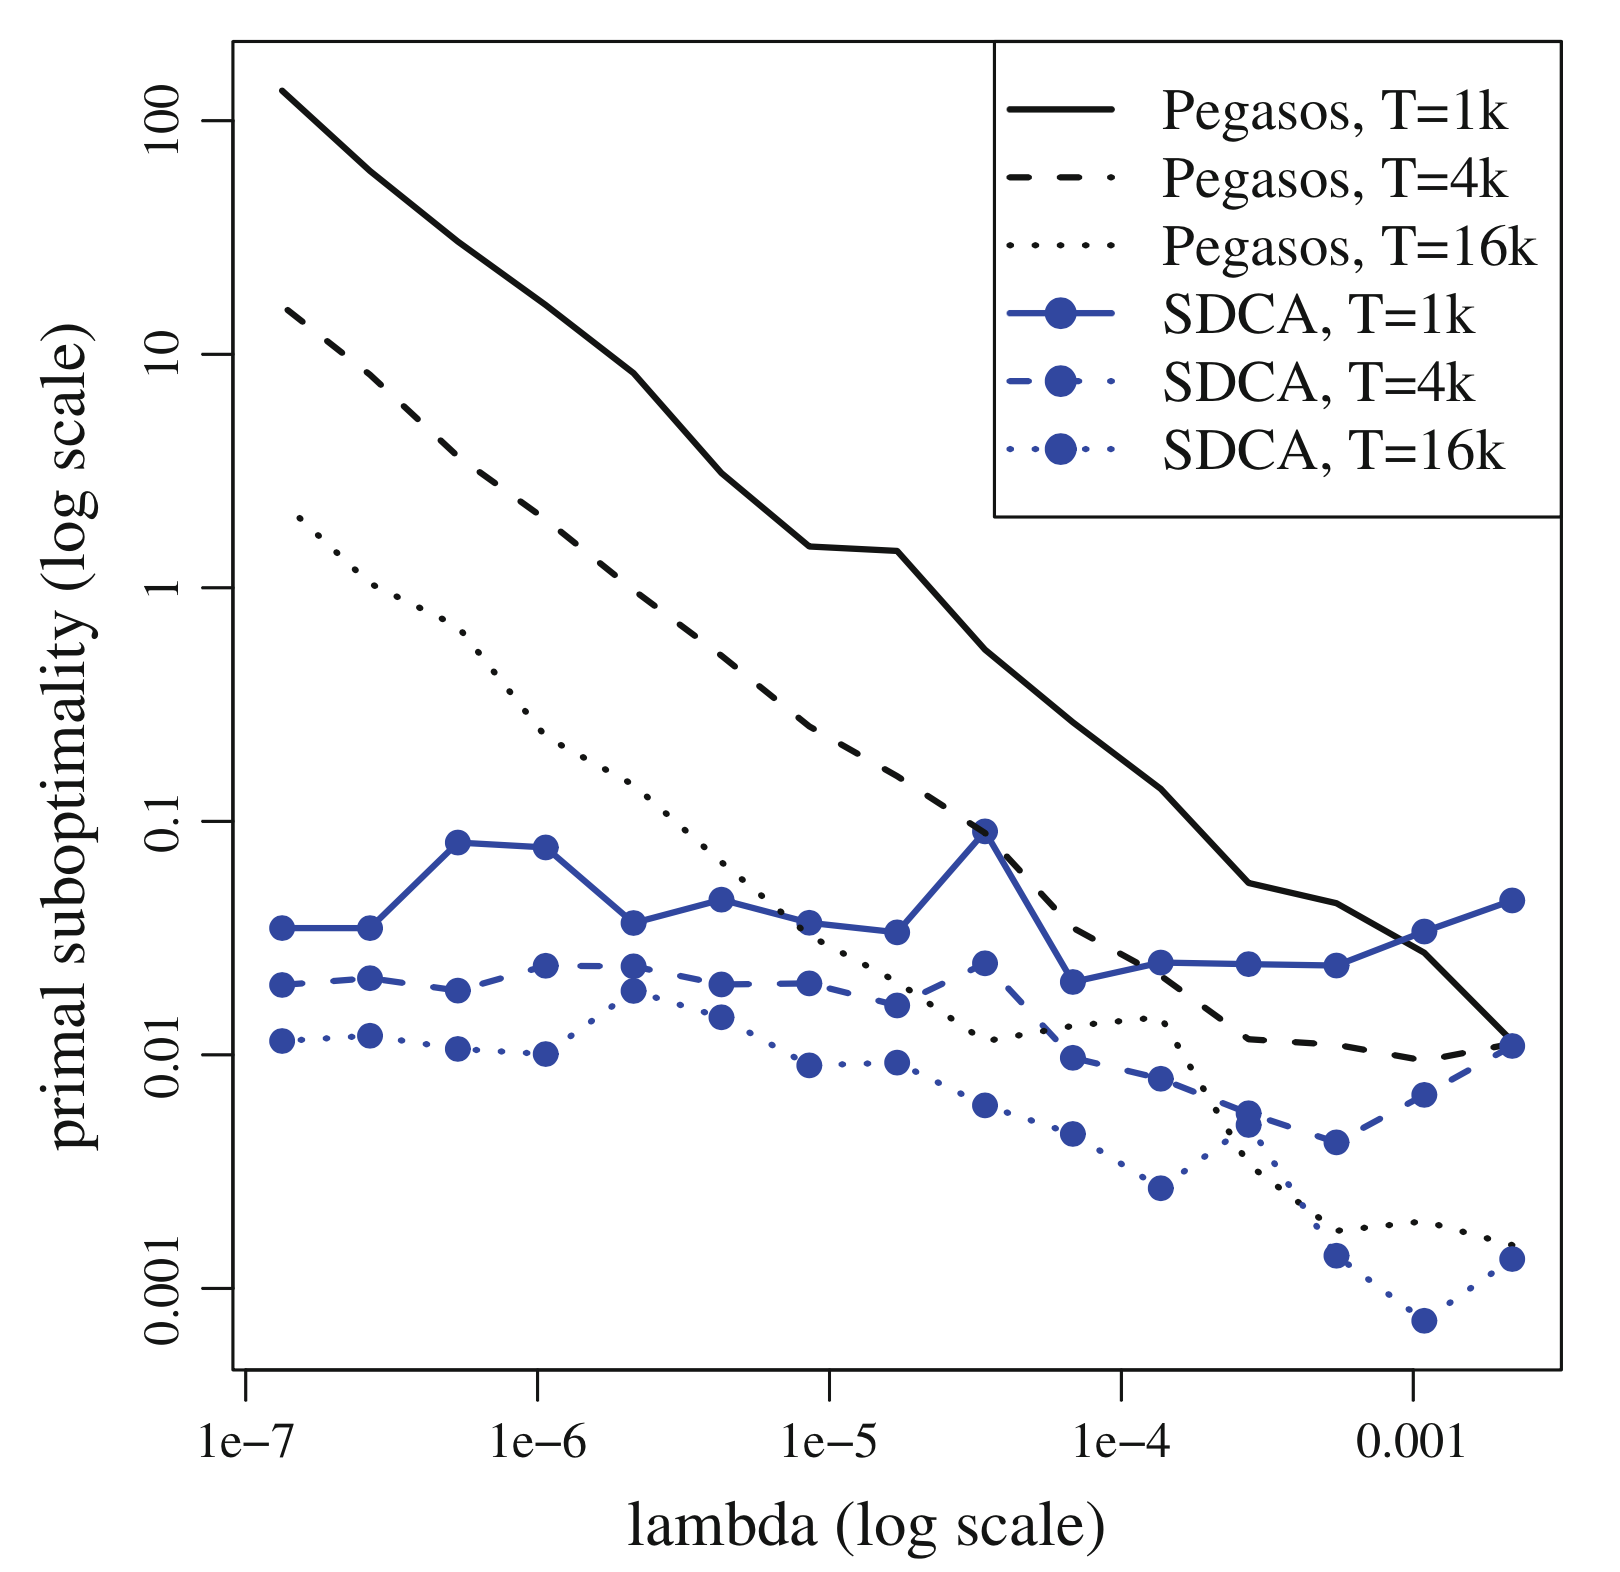
\includegraphics[height=0.7\textheight, width=0.7\textwidth]{images/comp_T.png}
    \end{figure}
\end{frame}

\begin{frame}{Experiments with the mini-batch variant}
    \begin{figure}[htbp]
        \centering
        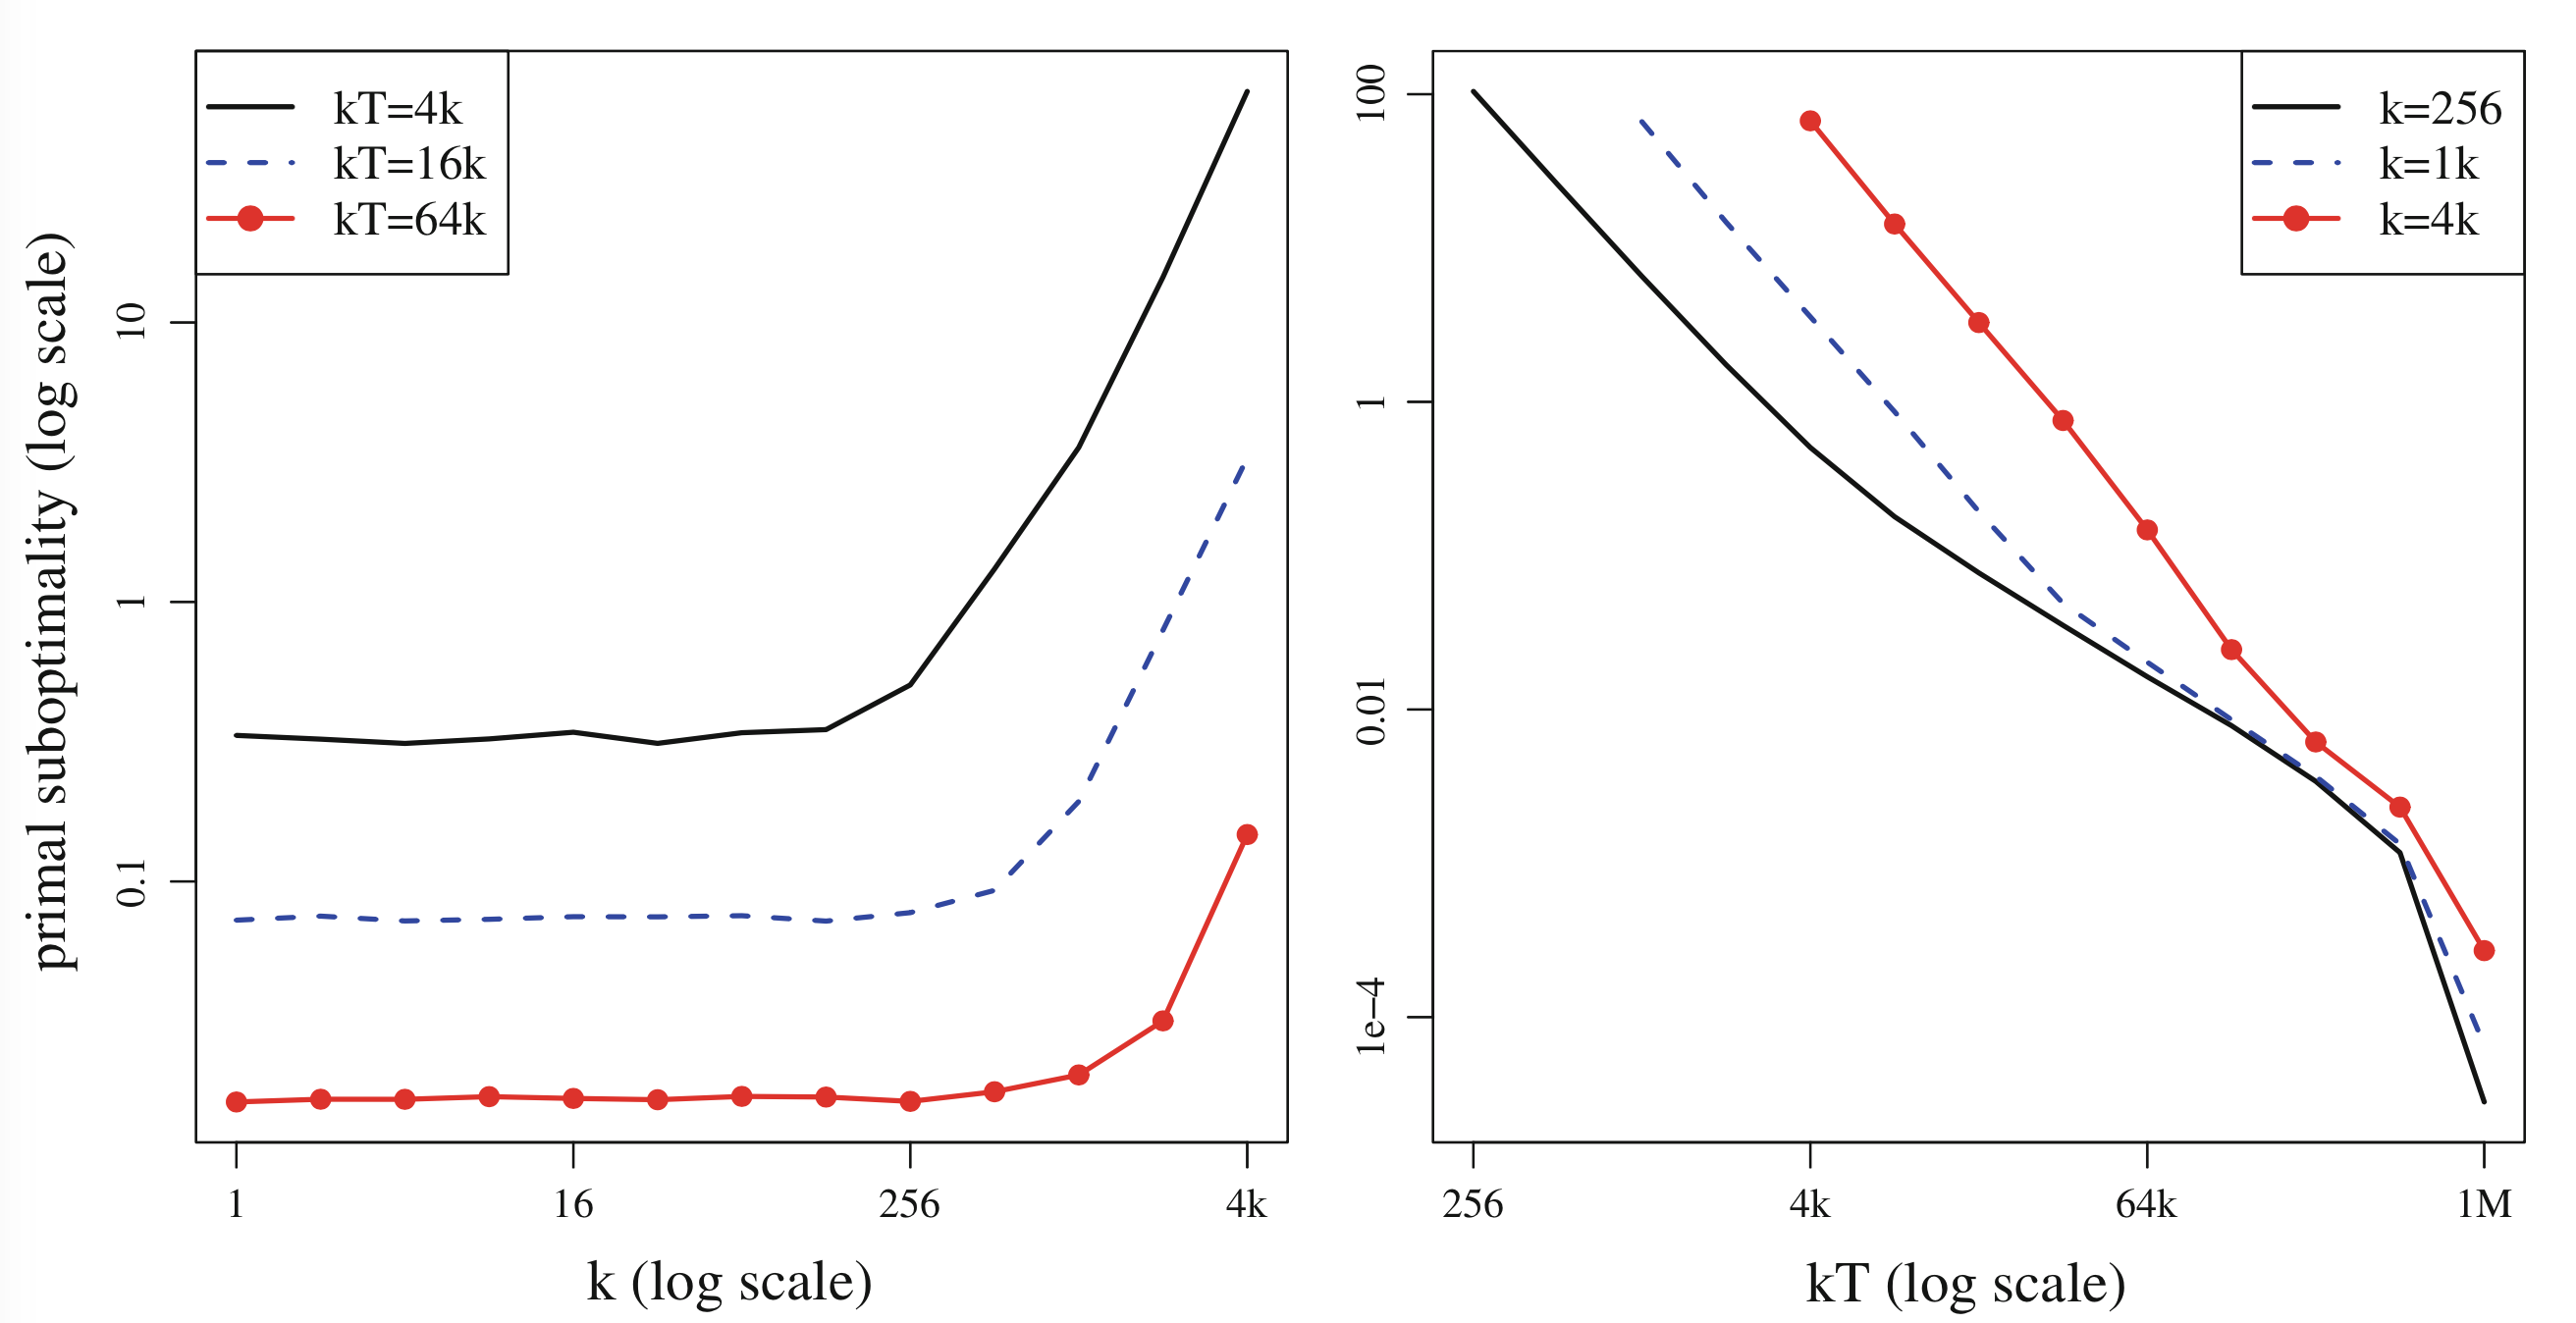
\includegraphics[height=0.7\textheight, width=\textwidth]{images/comp_nzh.png}
    \end{figure}
\end{frame}

\begin{frame}{Comparison of sampling procedures}
    \begin{figure}[htbp]
        \centering
        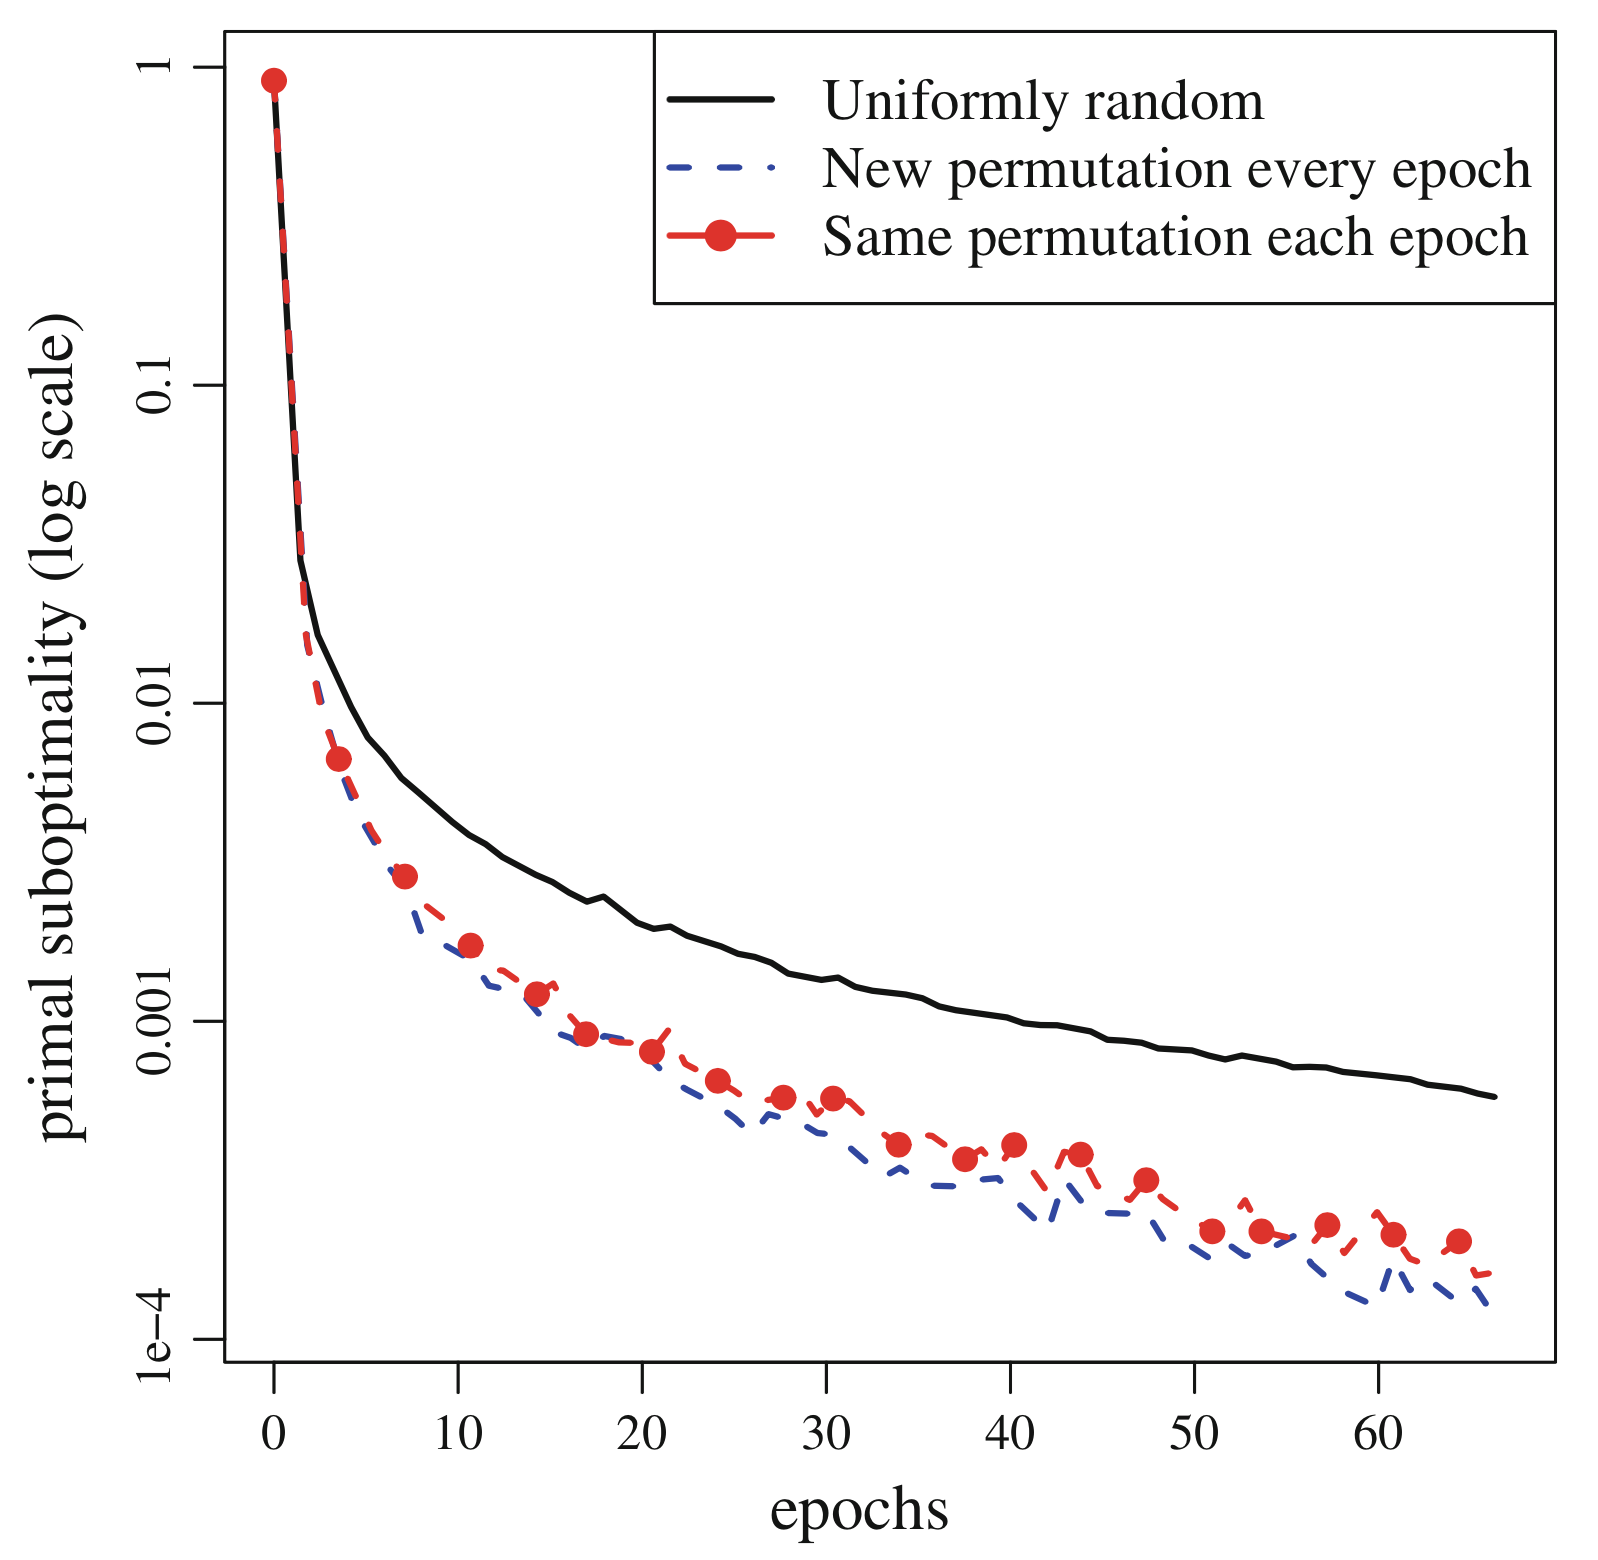
\includegraphics[height=0.7\textheight, width=0.7\textwidth]{images/epochs.png}
    \end{figure}
\end{frame}

\begin{frame}{Compare to Norma and Zhang (on Physics)}
    \begin{figure}[htbp]
        \centering
        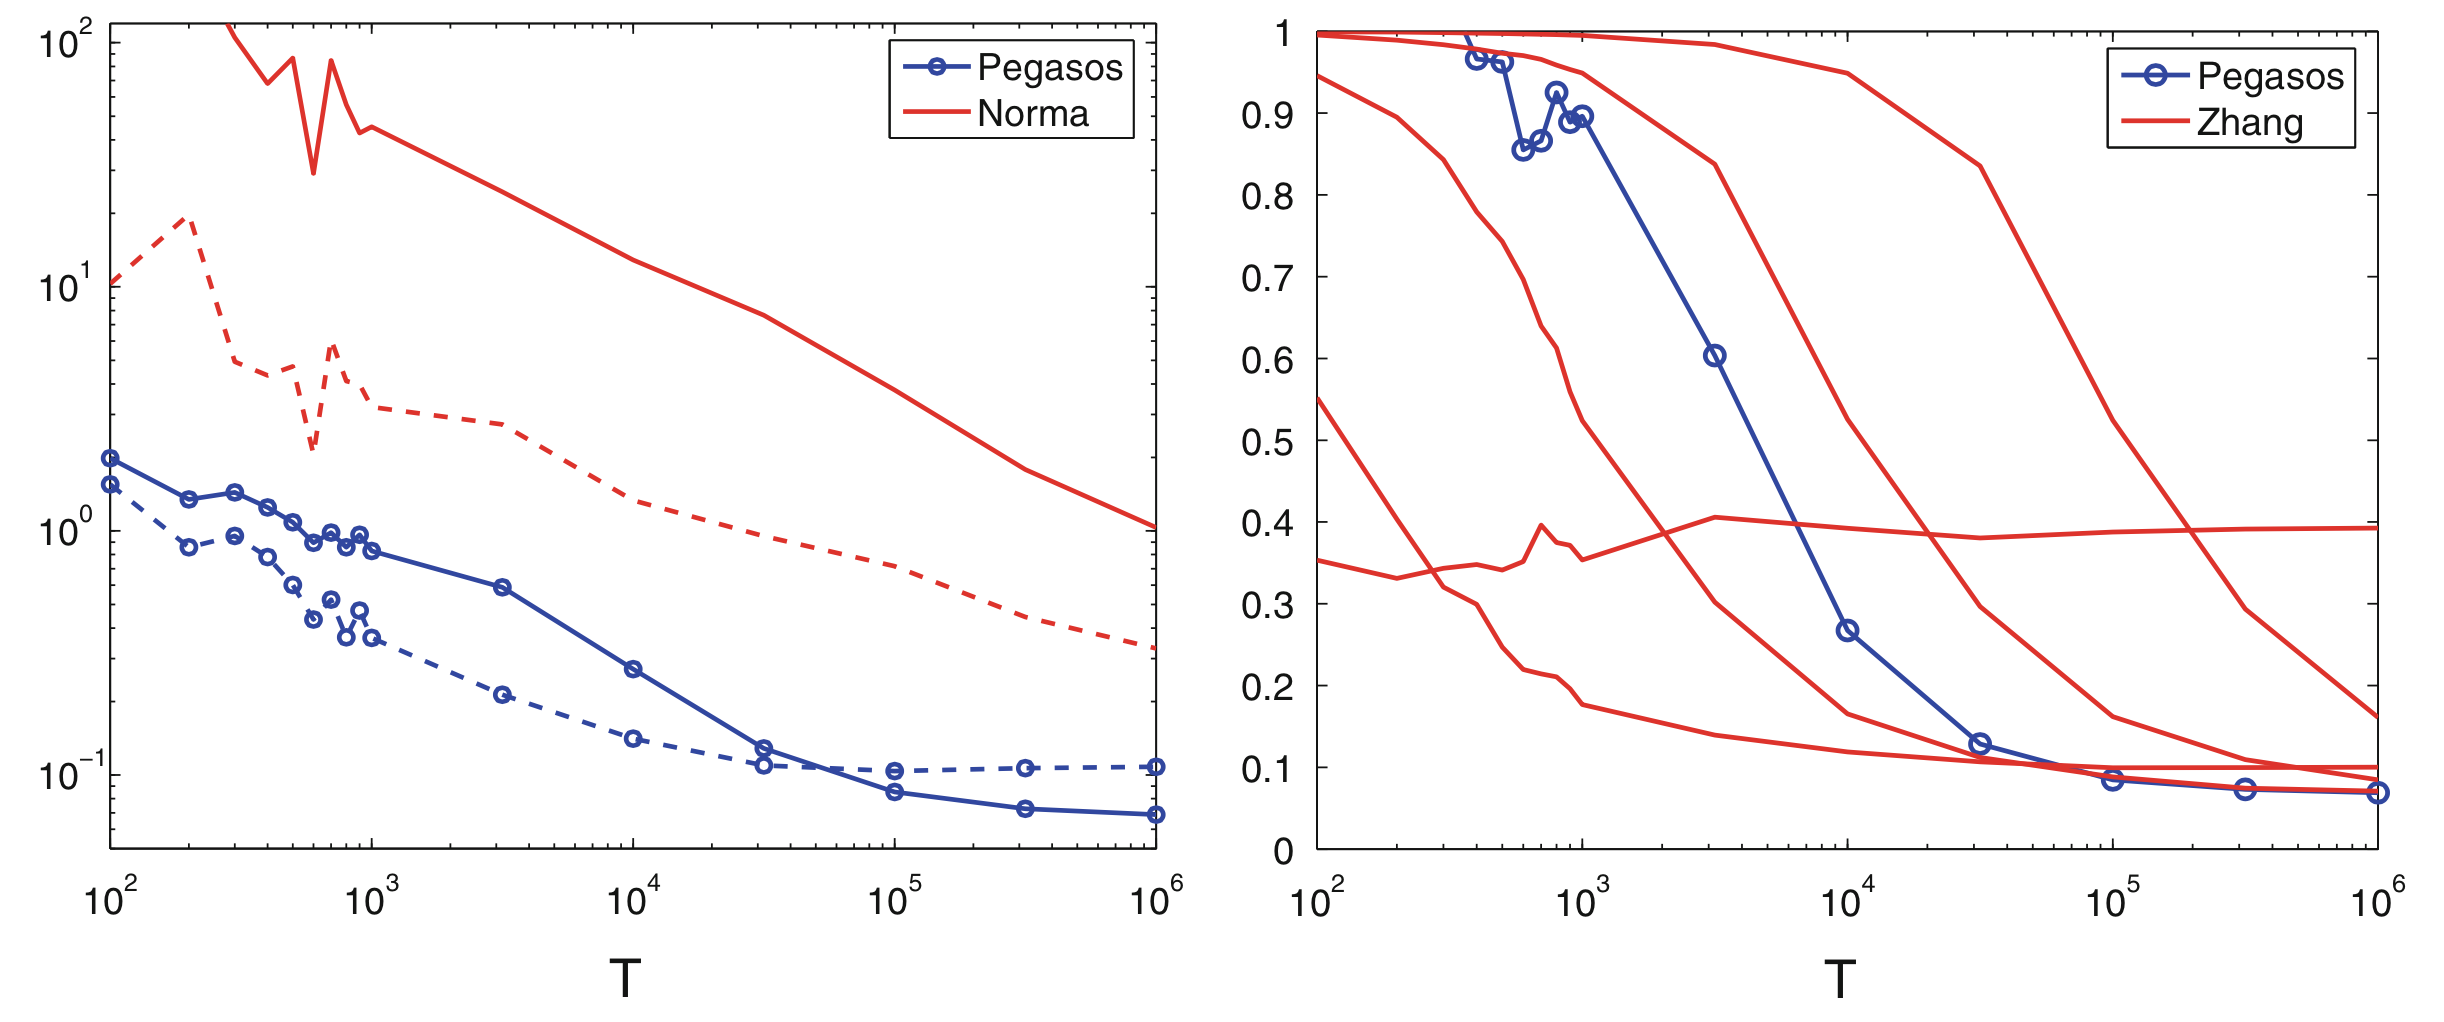
\includegraphics[height=0.7\textheight, width=\textwidth]{images/comp_k.png}
    \end{figure}
\end{frame}

\begin{frame}{Kernels}
    The basic Pegasos algorithm can easily be implemented using only kernel evaluations.
    \begin{itemize}
        \item For each t let $\mathbb{\alpha}_{t+1}\in R^n$ be the vector such that $\alpha_{t+1}[j]$ counts how many times example $j$ has been selected so far and we had a non-zero loss on it, namely, $\alpha_{t+1}[j]=\ |{t'\le t:i_{t'}=j\ \wedge\ y_j\langle \wv_{t'},\phi(\xv_j)\rangle < 1}|$.
        \item Represent $\wv_{t+1} = \frac{1}{\lambda t} \sum_{j=1}^{m} \alpha_{t+1}[j]y_j\phi(\xv_j)$
        \item {\color{green}Cons: overall runtime $\tilde{O}(nd/(\lambda \epsilon))$}
    \end{itemize}
\end{frame}

\begin{comment}
\begin{frame}{Bias term}
    \begin{enumerate}
        \item Popular approach: increase dimension of $x$

            {\color{green}Cons: ``pay'' for $b$ in the regularization term}
        \item Define: $L(\wv) = \min_b \sum_{(\xv,y)\in S} [1-y(\langle \wv, \xv\rangle - b)]_+$
        \item Rewrite problem: $\min_{\wv} {\frac{\lambda}{2}\|\wv\|^2+g(\wv;S)}$ where $g(\wv;S)=\min_b \frac1m \sum_{(\xv,y)\in S} \left[1-y(\langle \wv, \xv\rangle + b)\right]_+$

        Calculate subgradients w.r.t $w$ and w.r.t $b$.

        \item Search $b$ in an outer loop

            {\color{green}Cons: evaluation time remain same as unbiased}
    \end{enumerate}
\end{frame}
\end{comment}

\begin{frame}{Discussion}
    \begin{itemize}
        \item Pegasos: Simple $\&$ Efficient solver for SVM
        \item Sample vs. computational complexity
            \begin{itemize}
                \item Sample complexity: how many examples do we need as a function of VC-dim($\lambda$), accuracy($\epsilon$), and confidence($\delta$)
                \item In Pegasos, the authors aim at analyzing computational complexity based on $\lambda$, $\epsilon$, $\delta$ (also in Bottou $\&$ Bousquet)
            \end{itemize}
        \item Finding argmin vs. calculating min: It seems that Pegasos finds the argmin more easily than it requires to calculate the min value
    \end{itemize}
\end{frame}


\section{Reference}
\begin{frame}[fragile]
\frametitle{Reference}
\begin{itemize}
\item[] $\left[1\right]$ Shalev-Shwartz, Shai, et al. ``Pegasos: Primal estimated sub-gradient solver for svm.'' Mathematical programming 127.1 (2011): 3-30. 

\item[] $\left[2\right]$ Lacoste-Julien, Simon, Mark Schmidt, and Francis Bach. ``A simpler approach to obtaining an o (1/t) convergence rate for the projected stochastic subgradient method.'' arXiv preprint arXiv:1212.2002 (2012).

\item[] $\left[3\right]$  Tak\'a\v{c} Martin, et al. ``Mini-batch primal and dual methods for SVMs.'' arXiv preprint arXiv:1303.2314 (2013).
\item[] $\left[4\right]$ Zhao, Peilin, and Tong Zhang. ``Stochastic optimization with importance sampling.'' arXiv preprint arXiv:1401.2753 (2014).
\end{itemize}
\end{frame}

\begin{frame}{Q\&A}
\begin{figure}[htbp]
    \begin{multicols}{2}
    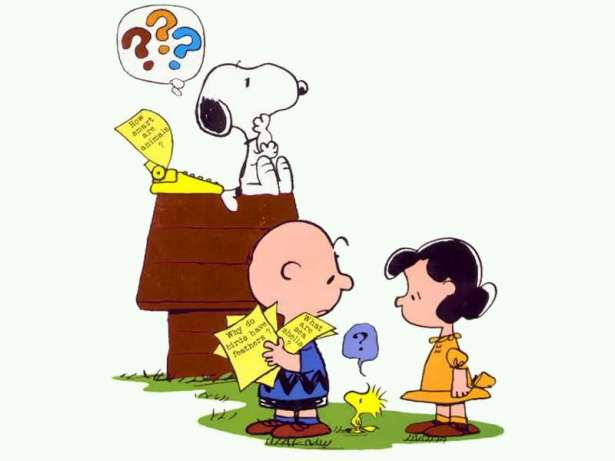
\includegraphics[height=0.4\textheight]{images/question.jpg}

    \Huge{Thank You!}
    \end{multicols}
\end{figure}

\textbf{Acknowledgement:}

Thanks to Martin for helpful discussions, suggestions and chips!!!

\end{frame}




\end{document}
